\begin{figure}[htbp]
\centering
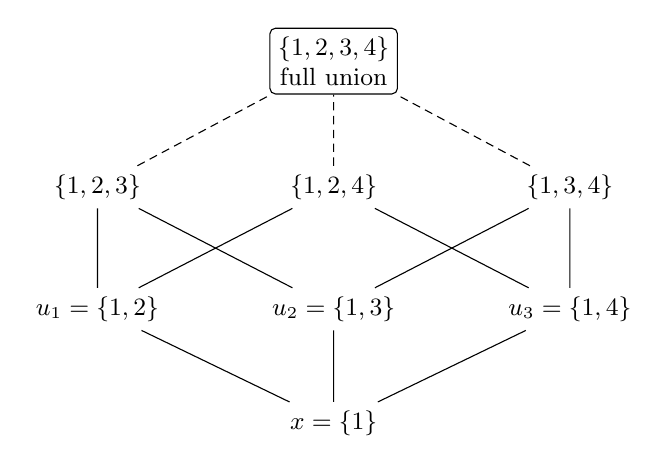
\begin{tikzpicture}[x=1cm,y=1cm,
  face/.style={fill=white,inner sep=3pt},
  every node/.style={font=\small}]
\node[face] (x) at (0,0) {$x=\{1\}$};
\node[face] (u1) at (-3,1.45) {$u_1=\{1,2\}$};
\node[face] (u2) at (0,1.45) {$u_2=\{1,3\}$};
\node[face] (u3) at (3,1.45) {$u_3=\{1,4\}$};
\node[face] (w12) at (-3,3) {$\{1,2,3\}$};
\node[face] (w13) at (0,3) {$\{1,2,4\}$};
\node[face] (w23) at (3,3) {$\{1,3,4\}$};
\node[face,draw,rounded corners=2pt,align=center] (all) at (0,4.6)
  {$\{1,2,3,4\}$\\full union};
\draw (x)--(u1) (x)--(u2) (x)--(u3);
\draw (u1)--(w12) (u1)--(w13);
\draw (u2)--(w12) (u2)--(w23);
\draw (u3)--(w13) (u3)--(w23);
\draw[densely dashed] (w12)--(all) (w13)--(all) (w23)--(all);
\end{tikzpicture}
\caption{The original Boolean faces containing $x$. Each pair among
$u_1,u_2,u_3$ has a proper union, but their total union is full.
All displayed subset relations survive the private insertions.
In the extension configuration of Proposition~\ref{ext:reduction},
solid edges correspond to restrictions of compatible homomorphisms
on actual nested domains. The dashed edges reach the full union,
for which a common extension is forbidden.}
\label{fig:boolean-faces}
\end{figure}
